%\documentclass[first,firstsupp,handout,compress,notes,navigation]{ETHclass} 
%\documentclass[first,firstsupp,handout,lastsupp]{ETHclass} 
\documentclass[first,firstsupp,lastsupp,handout,last,hyperref,table]{ETHclass} 
%\documentclass[first,firstsupp]{ETHclass}
\usepackage{etex}

\usepackage{adjustbox}
\usepackage{amsmath}
\usepackage{amssymb}
\usepackage{animate}
\usepackage{booktabs}
\usepackage{charter}
\usepackage{enumitem}
\usepackage{etoolbox}
\usepackage{ifthen}
\usepackage{longtable}
\usepackage{mathrsfs}
\usepackage{multicol}
\usepackage{pgf}
\usepackage{pgfplots}
\usepackage{pifont}
\usepackage{ragged2e}
\usepackage{standalone}
\usepackage[caption=false]{subfig}
\usepackage{tabularx}
\usepackage{tikz}
\usepackage{verbatim}
\usepackage{xcolor}
\usepackage{hyperref}

\pgfplotsset{compat=1.7}

\setbeamertemplate{navigation symbols}{}
\usetikzlibrary{arrows,decorations.pathreplacing,positioning,shapes,shadows}

%\usepackage[style=numeric-comp]{biblatex}

%\usepackage{lipsum}

%\usetikzlibrary{fit}
\usetikzlibrary{arrows}
\usetikzlibrary{trees}

% Options for beamer:
%
% 9,10,11,12,13,14,17pt  Fontsizes
% 
% compress: navigation bar becomes smaller
% t       : place contents of frames on top (alternative: b,c)
% handout : handoutversion
% notes   : show notes
% notes=onlyslideswithnotes
%
%hyperref={bookmarksopen,bookmarksnumbered} : Needed for menues in
%                                             acrobat. Also need
%                                             pdftex as option or 
%                                             compile with
% pdflatex '\PassOptionsToPackage{pdftex,bookmarksopen,bookmarksnumbered}{hyperref} \input{file}'

%\usepackage{beamerseminar}
%\usepackage[accumulated]{beamerseminar}
                                % remove ``accumulated'' option
                                % for original behaviour
%\usepackage{beamerbasenotes}
%\setbeamertemplate{note page}[plain] 
%\setbeameroption{notes on second screen}

%\setbeamertemplate{note page}[plain] 
\setbeamertemplate{note page}{\ \\[.3cm]
\textbf{\color{blue}Notes:}\\%[0.1cm]
{\footnotesize %\tiny
\insertnote}}
%\setbeameroption{notes on second screen}


%\setbeamertemplate{navigation symbols}{} % suppresses all navigation symbols:
 \setbeamertemplate{navigation symbols}[horizontal] % Organizes the navigation symbols horizontally.
% \setbeamertemplate{navigation symbols}[vertical] % Organizes the navigation symbols vertically.
% \setbeamertemplate{navigation symbols}[only frame symbol] % Shows only the navigational symbol for navigating frames.

\setlayoutscale{0.5}
\setparametertextfont{\scriptsize}
\setlabelfont{\scriptsize}

% \useoutertheme[subsection=false]{miniframes}
% \usepackage{etoolbox}
% \makeatletter
% \patchcmd{\slideentry}{\advance\beamer@xpos by1\relax}{}{}{}
% \def\beamer@subsectionentry#1#2#3#4#5{\advance\beamer@xpos by1\relax}%
% \makeatother

% \makeatletter
%     \newenvironment{withoutheadline}{
%        \setbeamertemplate{headline}{%
% \vspace{15pt}
% }
%     }{}
% \makeatother

\makeatletter
    \newenvironment{withoutheadline}{
         \setbeamertemplate{headline}{%
\vspace{35pt}
}
        %\def\beamer@entrycode{\vspace*{-1.5\headheight}}
    }{}
\makeatother

\newcommand{\Cross}{$\mathbin{\tikz [x=1.4ex,y=1.4ex,line width=.2ex, red] \draw (0,0) -- (1,1) (0,1) -- (1,0);}$}%

\newcommand{\Checkmark}{$\color{green}\checkmark$}

\setbeamerfont{subsection in toc}{size=\tiny}

\makeatletter
\patchcmd{\beamer@sectionintoc}
  {\vfill}
  {\vskip1.5\itemsep}
  {}
  {}
\makeatother  

\setbeamertemplate{frametitle continuation}{}

\setbeamertemplate{bibliography entry title}{}
\setbeamertemplate{bibliography entry author}{}
\setbeamertemplate{bibliography entry location}{}
\setbeamertemplate{bibliography entry note}{}

\setbeamercolor*{bibliography entry title}{fg=black}
\setbeamercolor*{bibliography entry author}{fg=black}
\setbeamercolor*{bibliography entry location}{fg=black}
\setbeamercolor*{bibliography entry note}{fg=black}
% and kill the abominable icon
%\setbeamertemplate{bibliography item}{\color{forestgreen}$\blacktriangleright$}
\setbeamertemplate{bibliography item}{\insertbiblabel}
%\setbeamertemplate{bibliography item}{\theenumiv}

\newcommand{\highlightred}[1]{%
  \colorbox{red!50}{$\displaystyle#1$}}
  
\newcommand{\highlightyellow}[1]{%
  \colorbox{yellow!50}{$\displaystyle#1$}}
  
\newcommand{\highlightgreen}[1]{%
  \colorbox{green!50}{$\displaystyle#1$}}

\AtBeginSection[]{
  \begin{frame}
  \vfill
  \centering
  \begin{beamercolorbox}[sep=8pt,center,shadow=true,rounded=true]{title}
    \usebeamerfont{frametitle}
\includegraphics[width=2ex]{freccia_trasparente_verde_foresta.png}\hspace{.5ex}~{\LARGE \textsc{\bfseries \insertsectionhead}}\par%
  \end{beamercolorbox}
  \vfill
  \end{frame}
}

\hyphenpenalty=5000
\tolerance=1000

\graphicspath{{figures/}}

\newenvironment{system}{\left\lbrace\begin{array}{@{}l@{}}}{\end{array}\right.}

\newenvironment{subsystem}{\left\lgroup\begin{array}{@{}l@{}}}{\end{array}\right.}

\defbeamertemplate*{title page}{customized}[1][]
{
\usebeamerfont{subtitle}
\usebeamercolor[fg]{subtitle}

\vspace{-1.75cm}

{\center
 \usebeamerfont{title}{\inserttitle}\par
}
\vspace{-.25cm}
{\flushleft
 \usebeamerfont{subtitle}{\small \insertsubtitle} \par
}

%\vspace{-.5cm}

{\center
\setbeamercolor{author}{bg=white,fg=Red}
\usebeamerfont{author}{\footnotesize \insertauthor} \par}

\vspace{-.2cm}

{\center
\usebeamerfont{institute}{\tiny \insertinstitute}\par }

\vspace{.2cm}

{\center
\usebeamerfont{date}{\scriptsize \insertdate} \par }

\vspace{0.2in}
}


\begin{document}
\setbeamertemplate{caption}{\raggedright\insertcaption\par}

\title{\textsc{Rapport d'avancement 2017-05-12}}
\author{ L. Di Stasio$^{1,2}$, Z. Ayadi$^{1}$, J. Varna$^{2}$}
%\institute{ Science et Ing\'enierie des Mat\'eriaux et M\'etallurgie (SI2M), Institut Jean Lamour, Nancy, France\\Department of Engineering Sciences and Mathematics, Division of Materials Science, Lule\aa\ University of Technology, Lule\aa, Sweden}
\institute{$^{1}$EEIGM, Universit\'e de Lorraine, Nancy, France\\$^{2}$Division of Materials Science, Lule\aa\ University of Technology, Lule\aa, Sweden}
\date{12 mai 2017}

\begin{frame}[plain]
    \titlepage
\end{frame}

\begin{withoutheadline}
\begin{frame}
\frametitle{Sommaire}
\justifying
\vspace*{-0.5cm}
% \tableofcontents[hidesubsections]
% \begin{multicols}{2}
% \tableofcontents[hidesubsections]
% \end{multicols}
% \begin{columns}[t]
%         \begin{column}{.5\textwidth}
%             \tableofcontents[sections={1-2}]
%         \end{column}
%         \begin{column}{.5\textwidth}
%             \tableofcontents[sections={3-6}]
%         \end{column}
%     \end{columns}
% \end{frame}
\tableofcontents[hidesubsections]
\end{frame}
\end{withoutheadline}

%\note{}

%\begin{frame}
%\pagediagram
%\end{frame}
%% \note{}

\section{Symboles, Mod\`eles \& Donn\'ees de R\'ef\'erence}

\subsection{Symboles}

\begin{frame}
\frametitle{Symboles}
\vspace{-0.25cm}
\footnotesize
\centering
\captionsetup[figure]{font=scriptsize,labelfont=scriptsize}
\begin{table}[htbp]

  \centering
  %\caption{Single phase properties summary.}
    \begin{tabularx}{\textwidth}{ccX}
    \textbf{Symbole}&\textbf{Unit\'e} & \textbf{Description} \\[3pt]
    \midrule\\[12pt]
	$\theta$ & $\left[^{\circ}\right]$ & Position du d\'ecollement, par rapport au centre de l'arc d\'efini par le d\'ecollement\\[1.5pt]
	$\Delta\theta$ & $\left[^{\circ}\right]$ & Ouverture angulaire du demi-d\'ecollement\\[4pt]
	$\delta$ & $\left[^{\circ}\right]$ & Angle sous-tendu par un seul \'el\'ement du maillage \'a l'interface fibre/matrice\\[3pt]
	$VF_{f}$ & $\left[-\right]$ & Fraction volumique des fibres\\[1.5pt]
	$l$ & $\left[\mu m\right]$ & Demi-\'epaisseur d'un pli, \'egal \'a la longuer du demi-cot\'e du VER (\'el\'ement carr\'e)\\[3pt]
	$u$ & $\left[\mu m\right]$ & D\'eplacement selon l'axe x\\[1.5pt]
	$w$ & $\left[\mu m\right]$ & D\'eplacement selon l'axe z\\
    \end{tabularx}%
  \label{tab:phaseprop}%
\end{table}%
\end{frame}

\begin{frame}
\frametitle{Symboles}
\vspace{-0.25cm}
\footnotesize
\centering
\captionsetup[figure]{font=scriptsize,labelfont=scriptsize}
\begin{table}[htbp]

  \centering
  %\caption{Single phase properties summary.}
    \begin{tabularx}{\textwidth}{ccX}
    \textbf{Symbole}&\textbf{Unit\'e} & \textbf{Description} \\[3pt]
    \midrule\\[12pt]
	$\Gamma_{1}$ & $\left[-\right]$ & Partie coll\'ee de la surface de la fibre\\[1.5pt]
	$\Gamma_{2}$ & $\left[-\right]$ & Partie d\'ecoll\'ee de la surface de la fibre\\[1.5pt]
	$\Gamma_{3}$ & $\left[-\right]$ & Partie coll\'ee de la surface de la matrice\\[1.5pt]
	$\Gamma_{4}$ & $\left[-\right]$ & Partie d\'ecoll\'ee de la surface de la matrice\\[1.5pt]
    \end{tabularx}%
  \label{tab:phaseprop}%
\end{table}%
\end{frame}

\subsection{Mod\`eles de R\'ef\'erence}

\begin{frame}
\frametitle{Mod\`eles de R\'ef\'erence}
\vspace{-0.25cm}
\centering
\begin{figure}
\centering
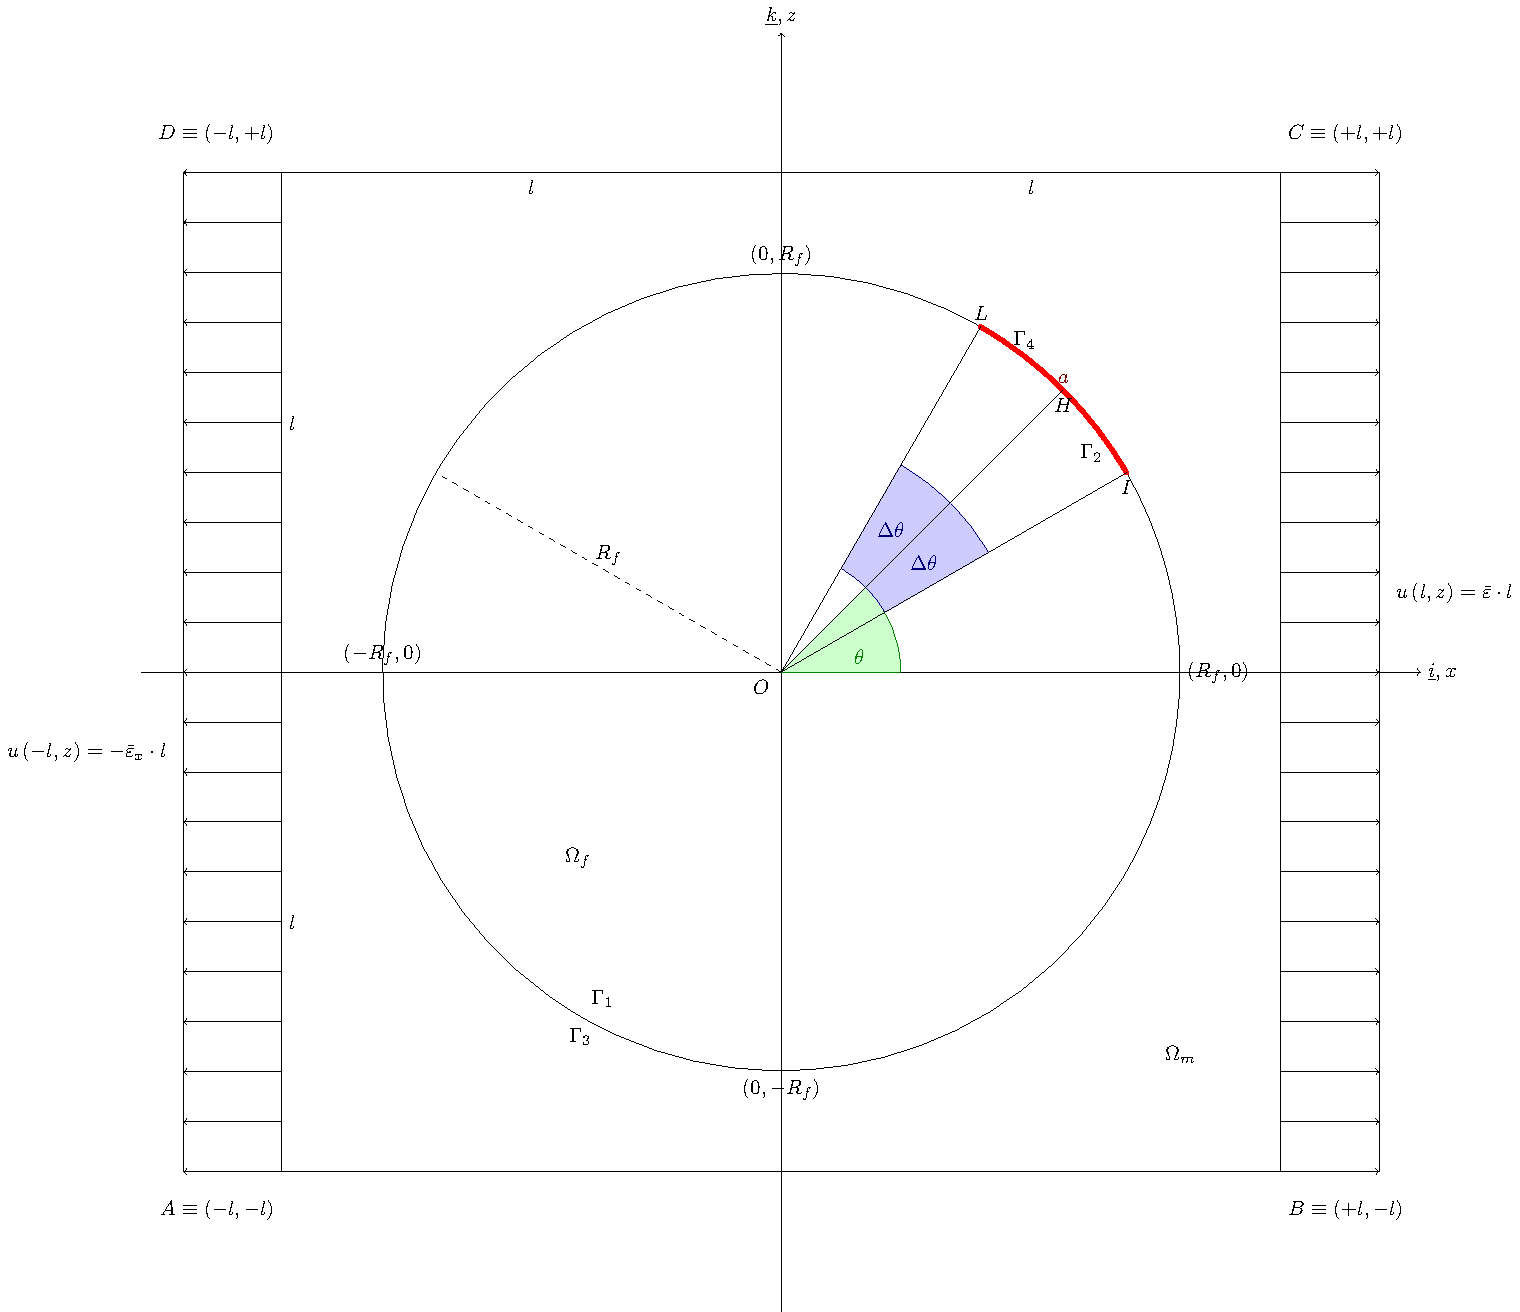
\includegraphics[height=0.7\textheight]{LEFM2DsRVEsFsDfreeBCULappAxialDispLR.pdf}
\caption{\scriptsize VER simple, conditions au bord: libre.}
\label{fig:singleRVE-rigid}
\end{figure}
\end{frame}

\begin{frame}
\frametitle{Mod\`eles de R\'ef\'erence}
\vspace{-0.25cm}
\centering
\begin{figure}
\centering
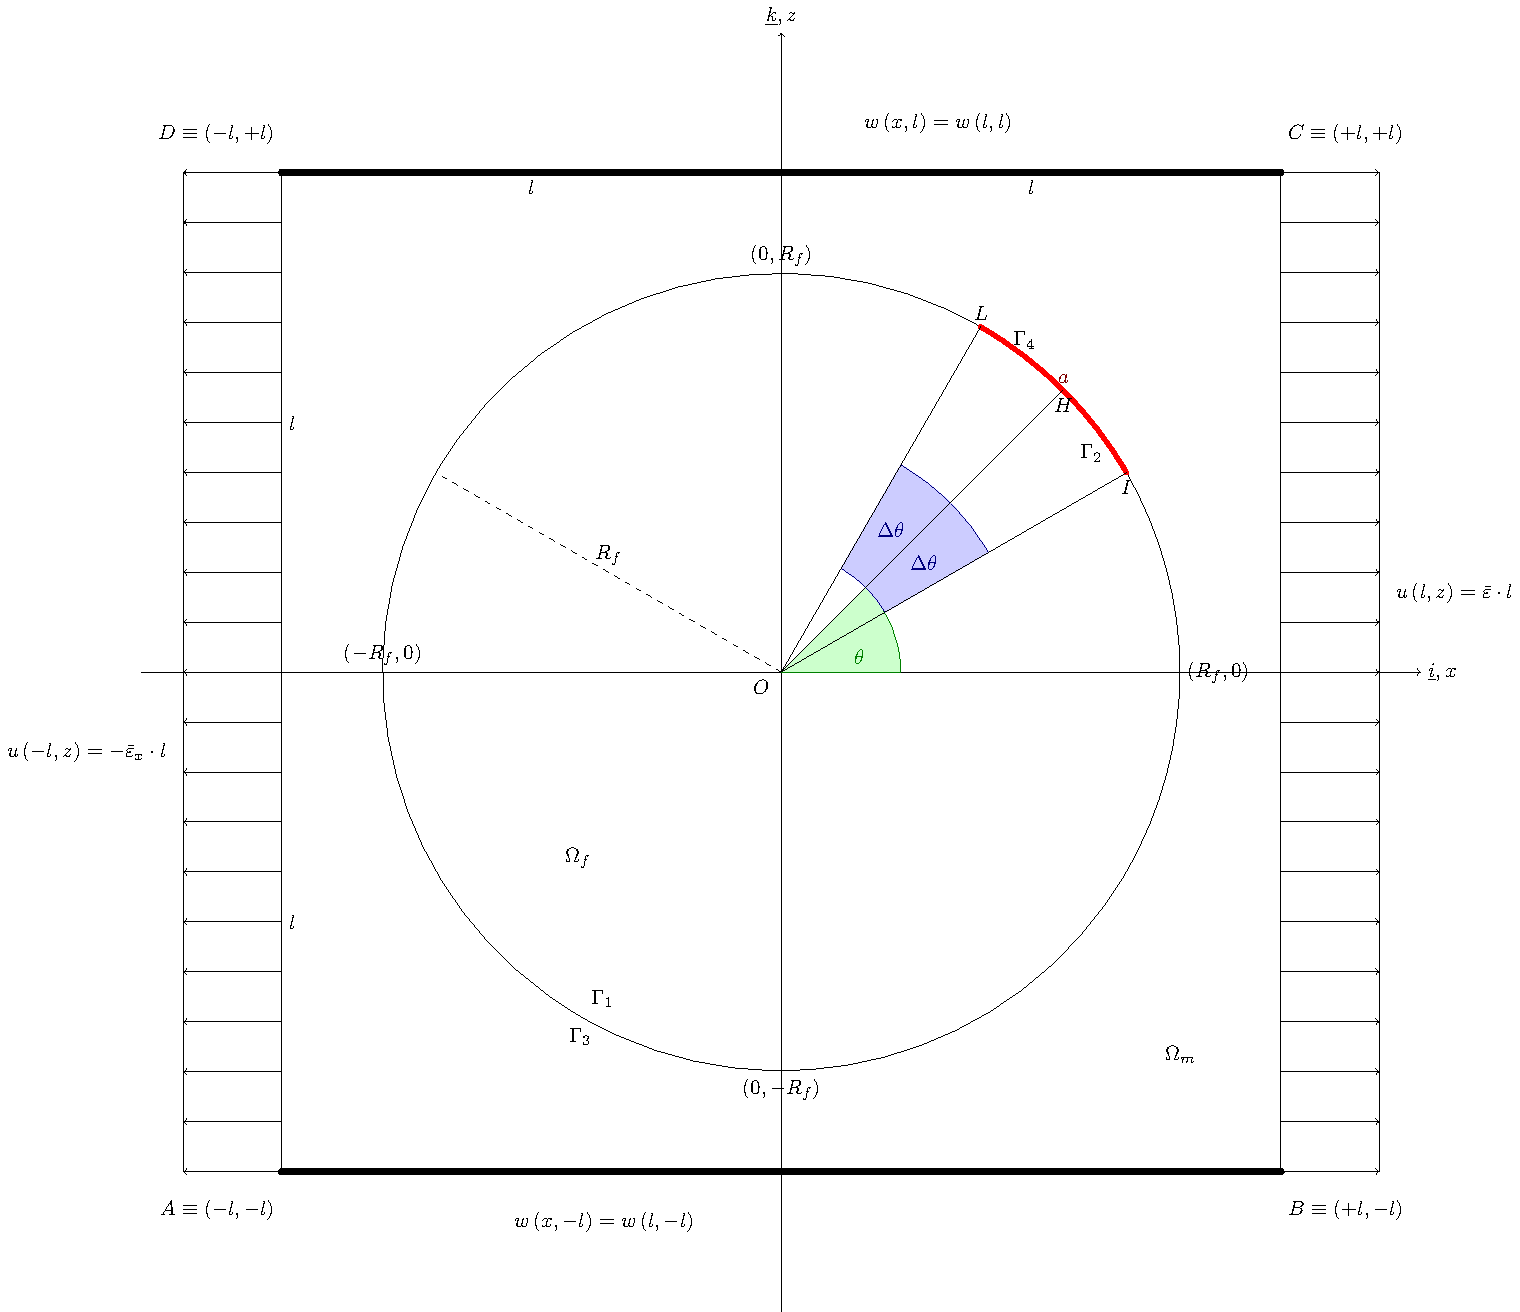
\includegraphics[height=0.7\textheight]{LEFM2DsRVEsFsDdepverdispBCULappAxialDispLR.pdf}
\caption{\scriptsize VER simple, conditions au bord: d\'eplacement vertical fix\'e.}
\label{fig:singleRVE-rigid}
\end{figure}
\end{frame}

\begin{frame}
\frametitle{Mod\`eles de R\'ef\'erence}
\vspace{-0.25cm}
\centering
\begin{figure}
\centering
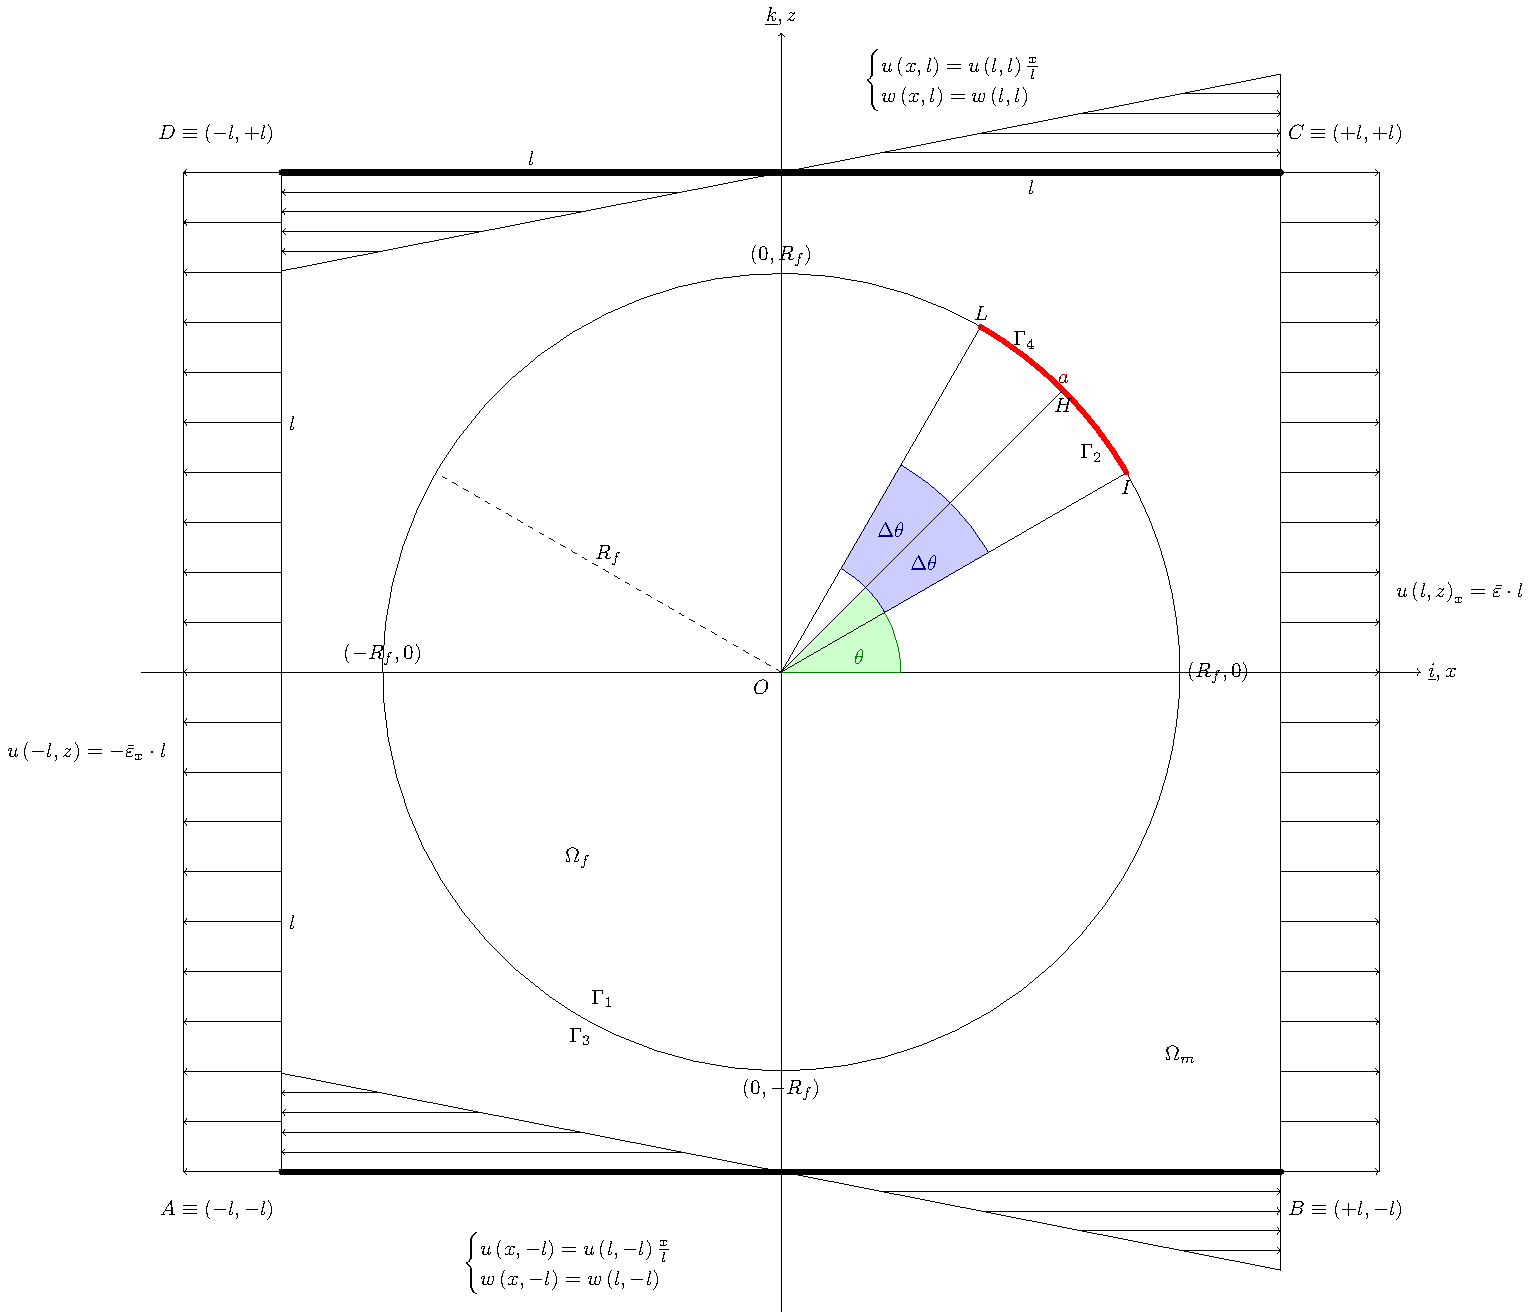
\includegraphics[height=0.7\textheight]{LEFM2DsRVEsFsDhomoBCULappAxialDispLR.pdf}
\caption{\scriptsize VER simple, conditions au bord: d\'eplacement vertical fix\'e et horizontal homog\'ene.}
\label{fig:singleRVE-homo}
\end{figure}
\end{frame}

\subsection{Discr\'etisation angulaire}

\begin{frame}
\frametitle{Discr\'etisation angulaire}
\vspace{-0.7cm}
\centering
\captionsetup[figure]{font=scriptsize,labelfont=scriptsize}
\begin{figure}[!h]
\centering
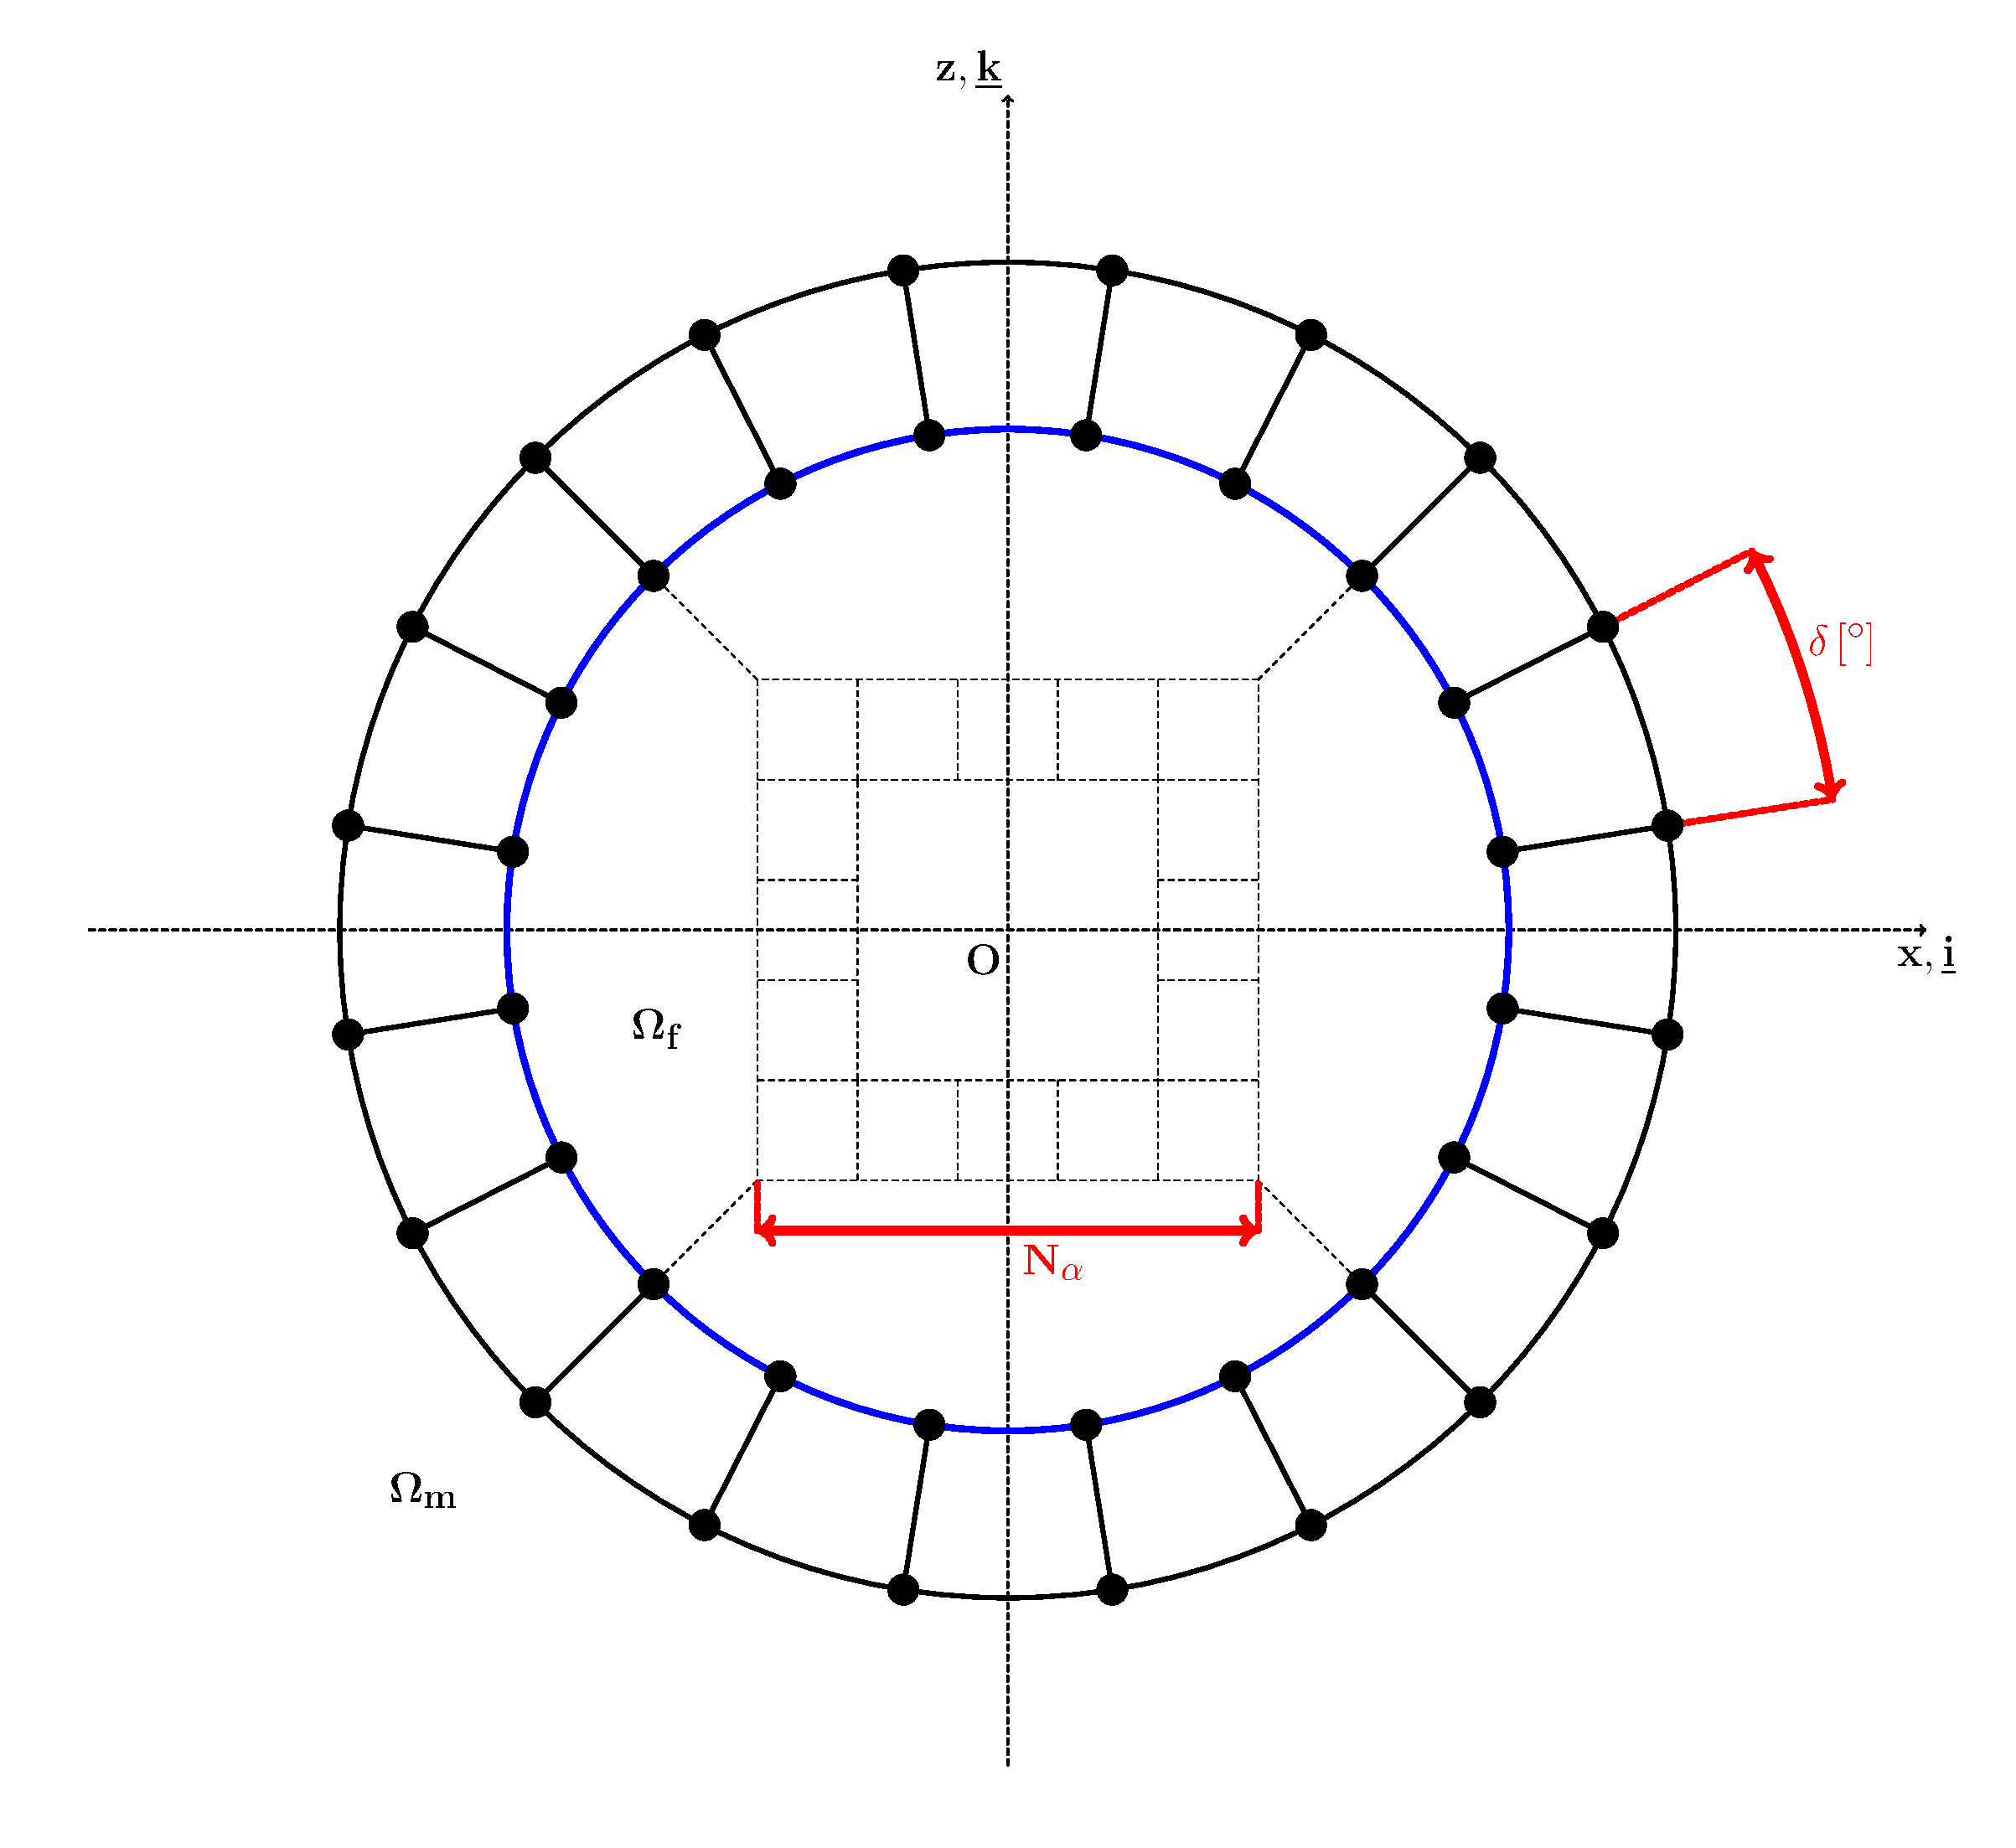
\includegraphics[height=0.7\textheight]{mesh-disc-at-interface.pdf}
  \caption{\scriptsize Discr\'etisation angulaire en correspondance de l'interface fibre/matrice: $\delta=\frac{360^{\circ}}{4N_{\alpha}}$.}
  \label{fig:angu-discr-def}
\end{figure}
\end{frame}

\subsection{Propri\'et\'es des mat\'eriaux}

\begin{frame}
\frametitle{Propri\'et\'es des mat\'eriaux}
\vspace{-0.7cm}
\footnotesize
\centering
\captionsetup[figure]{font=scriptsize,labelfont=scriptsize}
\begin{table}[htbp]

  \centering
  %\caption{Single phase properties summary.}
    \begin{tabular}{cccc}

    \textbf{Mat\'eriau} & \textbf{$E\left[GPa\right]$}\ & \textbf{$G\left[GPa\right]$} & \textbf{$\nu\left[-\right]$} \\[3pt]
    \midrule\\[12pt]
    Fibre de verre    & 70,0  & 29,2   & 0,2  \\[16pt]
    \'Epoxy    & 3,5    & 1,25   & 0,4  

    \end{tabular}%
  \label{tab:phaseprop}%
\end{table}%
\end{frame}

\section{D\'eveloppements \& travail r\'ealis\'e}

\subsection[R\'esultats obtenus]{R\'ecapitulation des r\'esultats obtenus}

\begin{frame}
\frametitle{R\'ecapitulation des r\'esultats obtenus}
\vspace{-0.25cm}
\scriptsize
\begin{list}{\Large\textcolor{green}{$\mathbf{\checkmark}$}}{}  
\item R\'eponse \'elastique globale correcte
\item Mod\`ele sym\'etrique donne r\'esultats sym\'etriques
\item Correct ordre de grandeur du taux de restitution d\'energie
\item R\'eponse correcte du rapport des modes: $G_{I}\uparrow\Delta\theta\downarrow$, $G_{II}\uparrow\Delta\theta\uparrow$
\item Pour $VF_{f}\to 0$ les conditions au bord n'ont aucun effets
\item La formulation de l'interface \'etais en effet sans friction
\end{list}
\begin{list}{\Huge\textcolor{red}{$\mathbf{\times}$}}{}  
\item Pas d'accord avec les r\'esultats du BEM  
\begin{itemize}[label=\ding{212}]
\item Taux de restitution d'\'energie surestim\'e
\item D\'ecalage des maximums de $\sim 10^{\circ}$
\end{itemize}
\end{list}
\end{frame}

\subsection[Objectifs]{R\'ecapitulation des objectifs}

\begin{frame}
\frametitle{R\'ecapitulation des objectifs}
\vspace{-0.5cm}
\vspace{-0.5cm}
\begin{list}{$\text{\rlap{\textcolor{white}{\huge$\mathbf{\checkmark}$}}}\square$}{}  
\item Changer la formulation de l'interface
\item Pour tester la formulation de l'interface, d\'evelopper mod\`ele de d\'ecollement entre deux demi-plans constitu\'es par deux diff\'erents mat\'eriaux
\end{list}
\end{frame}

\subsection{Travail r\'ealis\'e \& Actions \'a suivre}

\begin{frame}
\frametitle{Travail r\'ealis\'e \& Actions \'a suivre}
\vspace{-0.5cm}
\scriptsize
\begin{list}{$\text{\rlap{\textcolor{white}{\huge$\mathbf{\checkmark}$}}}\square$}{}  
\item Diff\'erentes formulations de l'interface (2/7)
\begin{itemize}[label=\ding{212}]
\item (Vieille formulation) 2 surfaces: $\text{surface de la fibre}=\Gamma_{1}+\Gamma_{2}$ et $\text{surface de la matrice}=\Gamma_{3}+\Gamma_{4}$ avec interaction $^{*}CONTACT$ et $^{*}DEBOND$ 
\end{itemize}
\begin{list}{$\text{\rlap{\textcolor{green}{\huge$\mathbf{\checkmark}$}}}\square$}{}  
\item 4 surfaces: $\Gamma_{1}$ sans les extr\'emit\'es de la fissure, $\Gamma_{2}$ avec les extr\'emit\'es de la fissure, $\Gamma_{3}$ sans les extr\'emit\'es de la fissure et $\Gamma_{4}$ avec les extr\'emit\'es de la fissure, interaction $*TIE$ entre  $\Gamma_{1}$ et $\Gamma_{3}$, interaction $^{*}CONTACT$ et $^{*}DEBOND$ entre  $\Gamma_{2}$ et $\Gamma_{4}$
\begin{list}{$\text{\rlap{\textcolor{green}{\huge$\mathbf{\checkmark}$}}}\square$}{}
\item D\'eveloppement du pr\'eprocesseur
\item Cr\'eation du mod\`ele MEF
\item Simulation param\'etrique
\item Analyse des r\'esultats
\end{list}
\end{list}
\end{list}
\end{frame}

\begin{frame}
\frametitle{Travail r\'ealis\'e \& Actions \'a suivre}
\vspace{-0.5cm}
\scriptsize
\begin{list}{$\text{\rlap{\textcolor{white}{\huge$\mathbf{\checkmark}$}}}\square$}{}  
\item Diff\'erentes formulations de l'interface (3/7)
\begin{list}{$\text{\rlap{\textcolor{green}{\huge$\mathbf{\checkmark}$}}}\square$}{}  
\item 2 surfaces: $\Gamma_{2}$ avec les extr\'emit\'es de la fissure et $\Gamma_{4}$ avec les extr\'emit\'es de la fissure, interaction $^{*}CONTACT$ et $^{*}DEBOND$ entre  $\Gamma_{2}$ et $\Gamma_{4}$, interaction $^{*}MPC\ TIE$ entre les \textit{points nodaux} de $\Gamma_{1}$ et $\Gamma_{3}$
\begin{list}{$\text{\rlap{\textcolor{green}{\huge$\mathbf{\checkmark}$}}}\square$}{}
\item D\'eveloppement du pr\'eprocesseur
\item Cr\'eation du mod\`ele MEF
\item Simulation param\'etrique
\item Analyse des r\'esultats
\end{list}
\end{list}
\end{list}
\end{frame}

\begin{frame}
\frametitle{Travail r\'ealis\'e \& Actions \'a suivre}
\vspace{-0.5cm}
\scriptsize
\begin{list}{$\text{\rlap{\textcolor{white}{\huge$\mathbf{\checkmark}$}}}\square$}{}  
\item Diff\'erentes formulations de l'interface (4/7)
\begin{list}{$\text{\rlap{\textcolor{white}{\huge$\mathbf{\checkmark}$}}}\square$}{}  
\item  4 surfaces: $\Gamma_{1}$ avec les extr\'emit\'es de la fissure, $\Gamma_{2}$ sans les extr\'emit\'es de la fissure, $\Gamma_{3}$ avec les extr\'emit\'es de la fissure et $\Gamma_{4}$ sans les extr\'emit\'es de la fissure, interaction $^{*}TIE$ entre  $\Gamma_{1}$ et $\Gamma_{3}$, interaction $^{*}CONTACT$ entre  $\Gamma_{2}$ et $\Gamma_{4}$
\begin{list}{$\text{\rlap{\textcolor{green}{\huge$\mathbf{\checkmark}$}}}\square$}{}
\item D\'eveloppement du pr\'eprocesseur
\item Cr\'eation du mod\`ele MEF
\item Simulation param\'etrique
\end{list}
\begin{list}{$\text{\rlap{\textcolor{white}{\huge$\mathbf{\checkmark}$}}}\square$}{}  
\item Mise en oeuvre du VCCT dans le postprocesseur
\item Analyse des r\'esultats
\end{list}
\end{list}
\end{list}
\end{frame}

\begin{frame}
\frametitle{Travail r\'ealis\'e \& Actions \'a suivre}
\vspace{-0.5cm}
\scriptsize
\begin{list}{$\text{\rlap{\textcolor{white}{\huge$\mathbf{\checkmark}$}}}\square$}{}  
\item Diff\'erentes formulations de l'interface (5/7)
\begin{list}{$\text{\rlap{\textcolor{white}{\huge$\mathbf{\checkmark}$}}}\square$}{}  
\item  2 surfaces: $\Gamma_{2}$ sans les extr\'emit\'es de la fissure et $\Gamma_{4}$ sans les extr\'emit\'es de la fissure, interaction $^{*}CONTACT$ entre  $\Gamma_{2}$ et $\Gamma_{4}$, interaction $^{*}MPC\ TIE$ entre les \textit{points nodaux} de $\Gamma_{1}$ et $\Gamma_{3}$
\begin{list}{$\text{\rlap{\textcolor{green}{\huge$\mathbf{\checkmark}$}}}\square$}{}
\item D\'eveloppement du pr\'eprocesseur
\item Cr\'eation du mod\`ele MEF
\item Simulation param\'etrique
\end{list}
\begin{list}{$\text{\rlap{\textcolor{white}{\huge$\mathbf{\checkmark}$}}}\square$}{}  
\item Mise en oeuvre du VCCT dans le postprocesseur
\item Analyse des r\'esultats
\end{list}
\end{list}
\end{list}
\end{frame}

\begin{frame}
\frametitle{Travail r\'ealis\'e \& Actions \'a suivre}
\vspace{-0.5cm}
\scriptsize
\begin{list}{$\text{\rlap{\textcolor{white}{\huge$\mathbf{\checkmark}$}}}\square$}{}  
\item Diff\'erentes formulations de l'interface (6/7)
\begin{list}{$\text{\rlap{\textcolor{white}{\huge$\mathbf{\checkmark}$}}}\square$}{}  
\item  2 surfaces: $\Gamma_{2}$ sans les extr\'emit\'es de la fissure et $\Gamma_{4}$ sans les extr\'emit\'es de la fissure, interaction $^{*}CONTACT$ entre  $\Gamma_{2}$ et $\Gamma_{4}$, interaction $^{*}EQUATION$ entre les \textit{points nodaux} de $\Gamma_{1}$ et $\Gamma_{3}$ avec \textit{dummy node} pour mesurer la force de r\'eaction
\begin{list}{$\text{\rlap{\textcolor{white}{\huge$\mathbf{\checkmark}$}}}\square$}{}  
\item D\'eveloppement du pr\'eprocesseur
\item Cr\'eation du mod\`ele MEF
\item Simulation param\'etrique
\item Mise en oeuvre du VCCT dans le postprocesseur
\item Analyse des r\'esultats
\end{list}
\end{list}
\end{list}
\end{frame}

\begin{frame}
\frametitle{Travail r\'ealis\'e \& Actions \'a suivre}
\vspace{-0.5cm}
\scriptsize
\begin{list}{$\text{\rlap{\textcolor{white}{\huge$\mathbf{\checkmark}$}}}\square$}{}  
\item Diff\'erentes formulations de l'interface (7/7)
\begin{list}{$\text{\rlap{\textcolor{white}{\huge$\mathbf{\checkmark}$}}}\square$}{}  
\item  2 surfaces: $\Gamma_{2}$ sans les extr\'emit\'es de la fissure et $\Gamma_{4}$ sans les extr\'emit\'es de la fissure, interaction $^{*}CONTACT$ entre  $\Gamma_{2}$ et $\Gamma_{4}$, interaction $^{*}CONN2D2\ TIE$ entre les \textit{points nodaux} de $\Gamma_{1}$ et $\Gamma_{3}$
\begin{list}{$\text{\rlap{\textcolor{white}{\huge$\mathbf{\checkmark}$}}}\square$}{}  
\item D\'eveloppement du pr\'eprocesseur
\item Cr\'eation du mod\`ele MEF
\item Simulation param\'etrique
\item Mise en oeuvre du VCCT dans le postprocesseur
\item Analyse des r\'esultats
\end{list}
\end{list}
\end{list}
\end{frame}

\begin{frame}
\frametitle{Travail r\'ealis\'e \& Actions \'a suivre}
\vspace{-0.5cm}
\scriptsize
\begin{list}{$\text{\rlap{\textcolor{white}{\huge$\mathbf{\checkmark}$}}}\square$}{}  
\item Pour tester la formulation de l'interface, d\'evelopper mod\`ele de d\'ecollement entre deux demi-plans constitu\'es par deux diff\'erents mat\'eriaux
\begin{list}{$\text{\rlap{\textcolor{green}{\huge$\mathbf{\checkmark}$}}}\square$}{}
\item D\'eveloppement du pr\'eprocesseur
\end{list}
\begin{list}{$\text{\rlap{\textcolor{white}{\huge$\mathbf{\checkmark}$}}}\square$}{}
\item Cr\'eation du mod\`ele MEF
\item Simulation param\'etrique
\item Mise en oeuvre du VCCT dans le postprocesseur
\item Analyse des r\'esultats
\end{list}
\end{list}
\end{frame}

\subsection{R\'esultats}

\begin{frame}
\frametitle{R\'esultats}
\vspace{-0.7cm}
\centering
\captionsetup[figure]{font=scriptsize,labelfont=scriptsize}
\begin{figure}[!h]
\centering
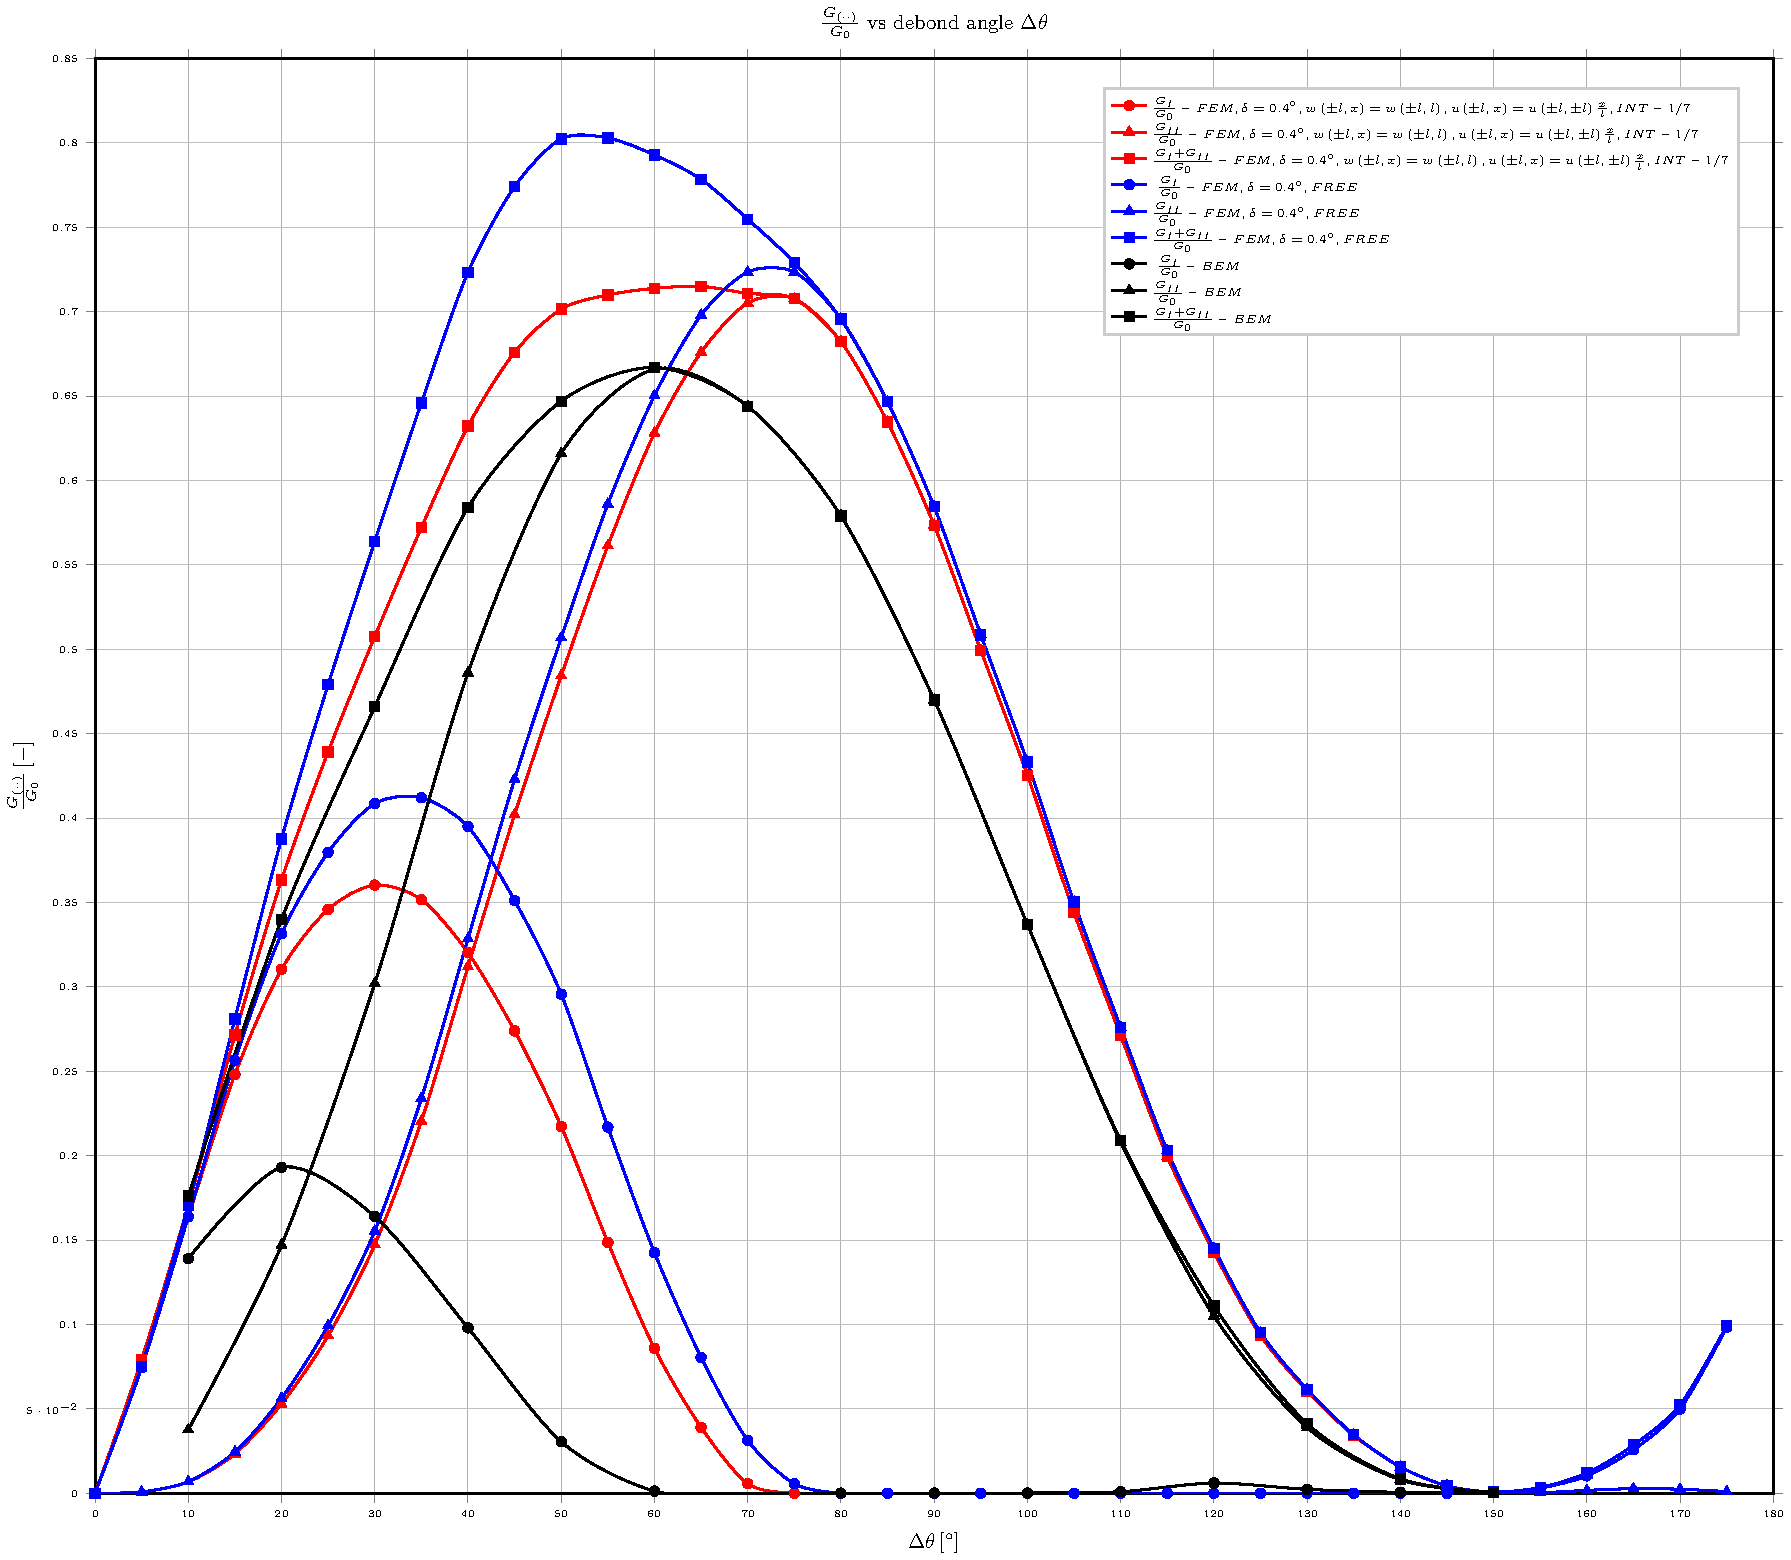
\includegraphics[height=0.7\textheight]{2017-04-29_AbqRunSummary_GsoverG0_FEM-BEM-comparison.pdf}
  \caption{\scriptsize Formulation de l'interface 2/7.}
  \label{fig:res1}
\end{figure}
\end{frame}

\begin{frame}
\frametitle{R\'esultats}
\vspace{-0.7cm}
\centering
\captionsetup[figure]{font=scriptsize,labelfont=scriptsize}
\begin{figure}[!h]
\centering
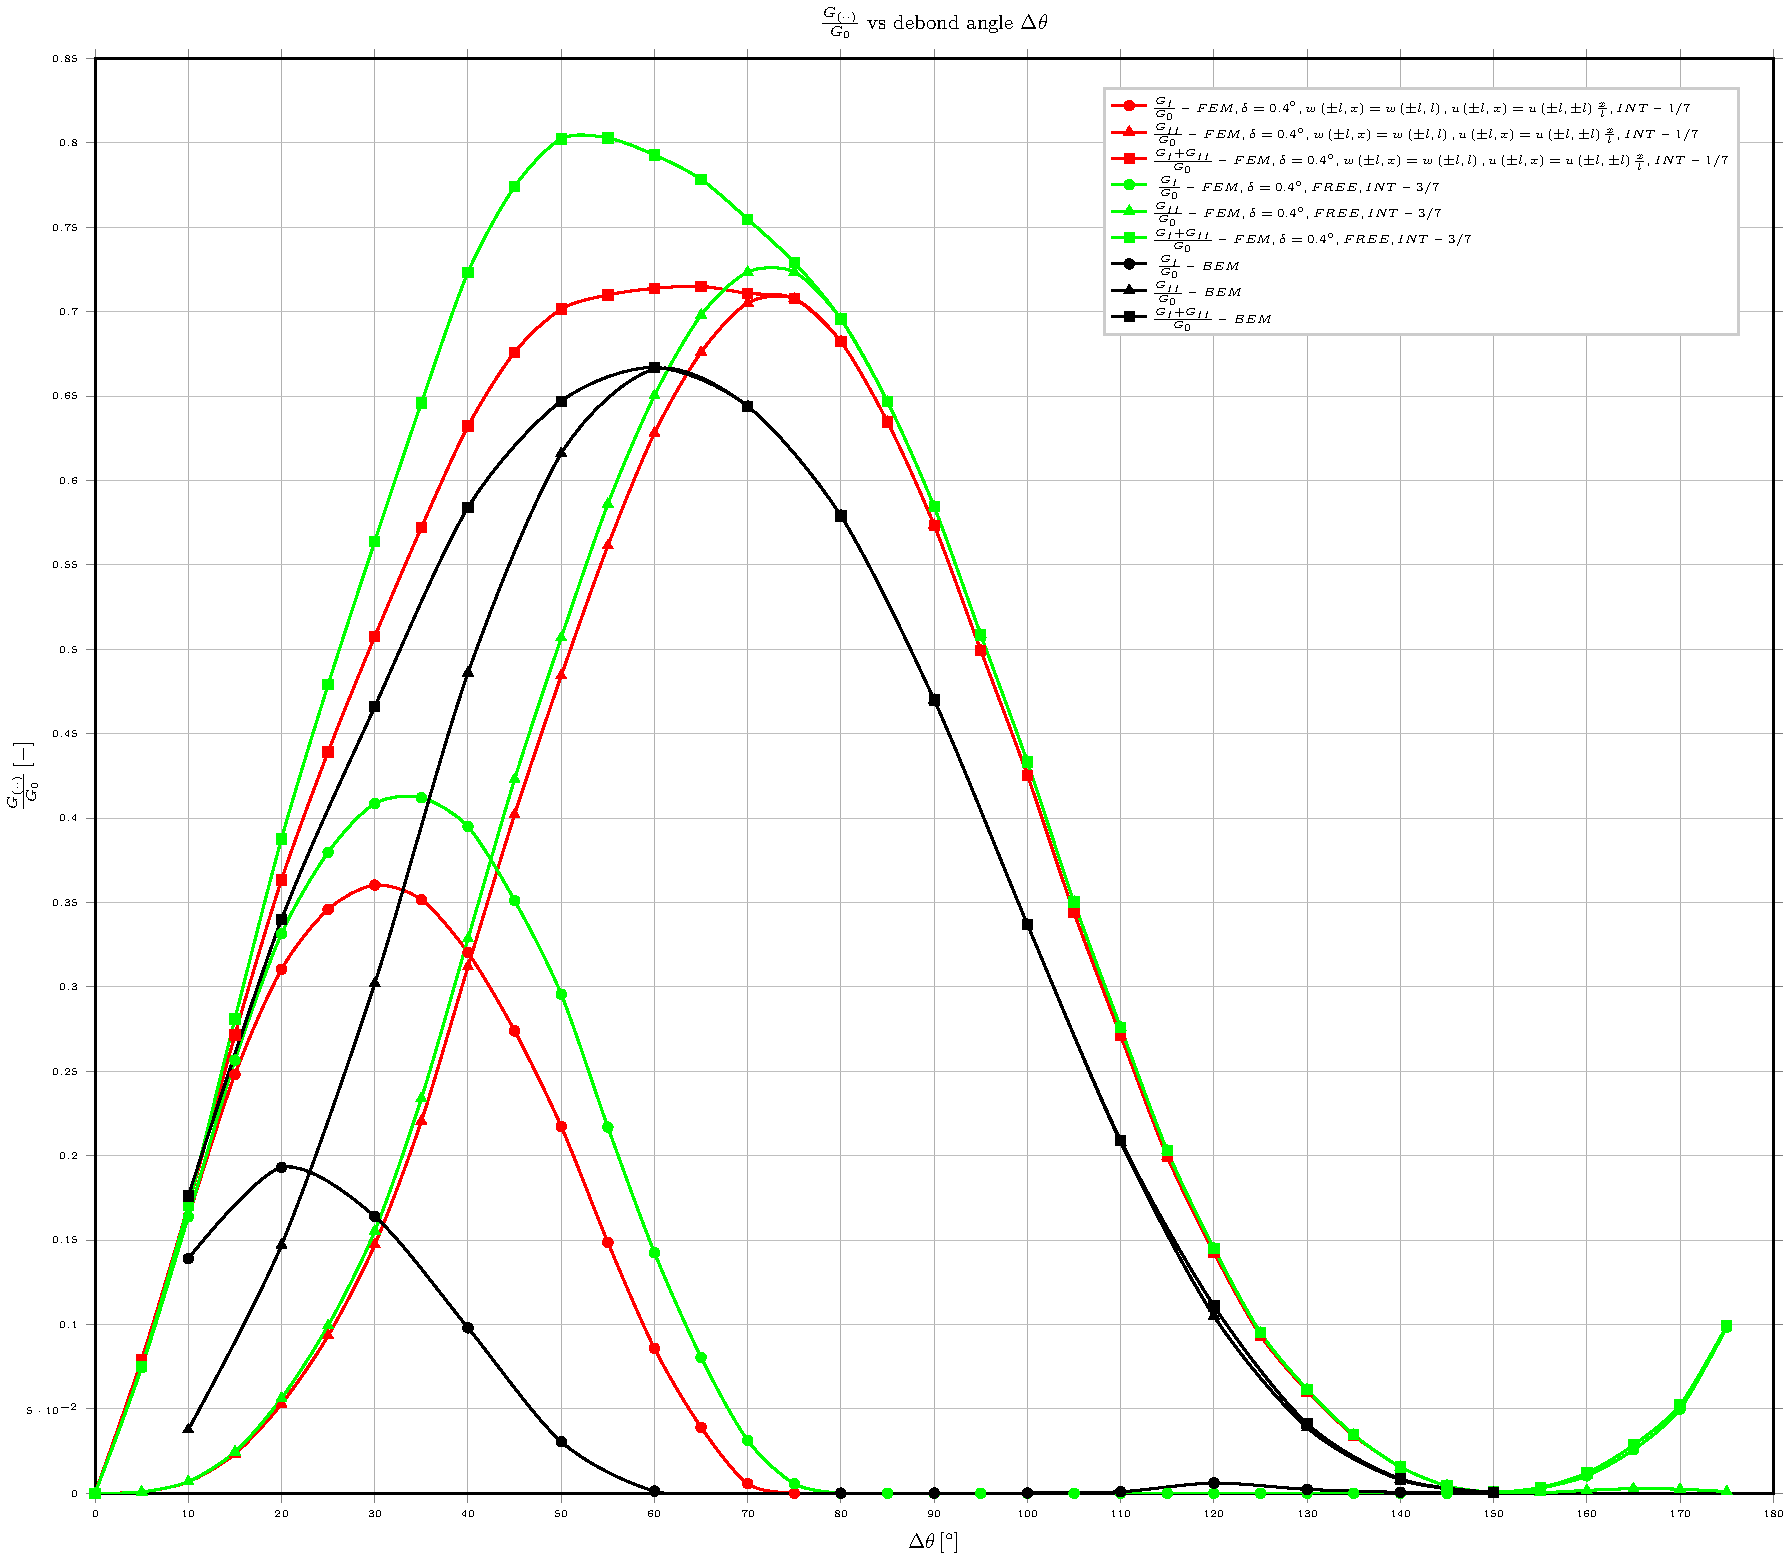
\includegraphics[height=0.7\textheight]{2017-05-03_AbqRunSummary_GsoverG0_FEM-BEM-comparison.pdf}
  \caption{\scriptsize Formulation de l'interface 3/7.}
  \label{fig:res1}
\end{figure}
\end{frame}

\begin{frame}
\frametitle{R\'esultats}
\vspace{-0.7cm}
\centering
\captionsetup[figure]{font=scriptsize,labelfont=scriptsize}
\begin{figure}[!h]
\centering
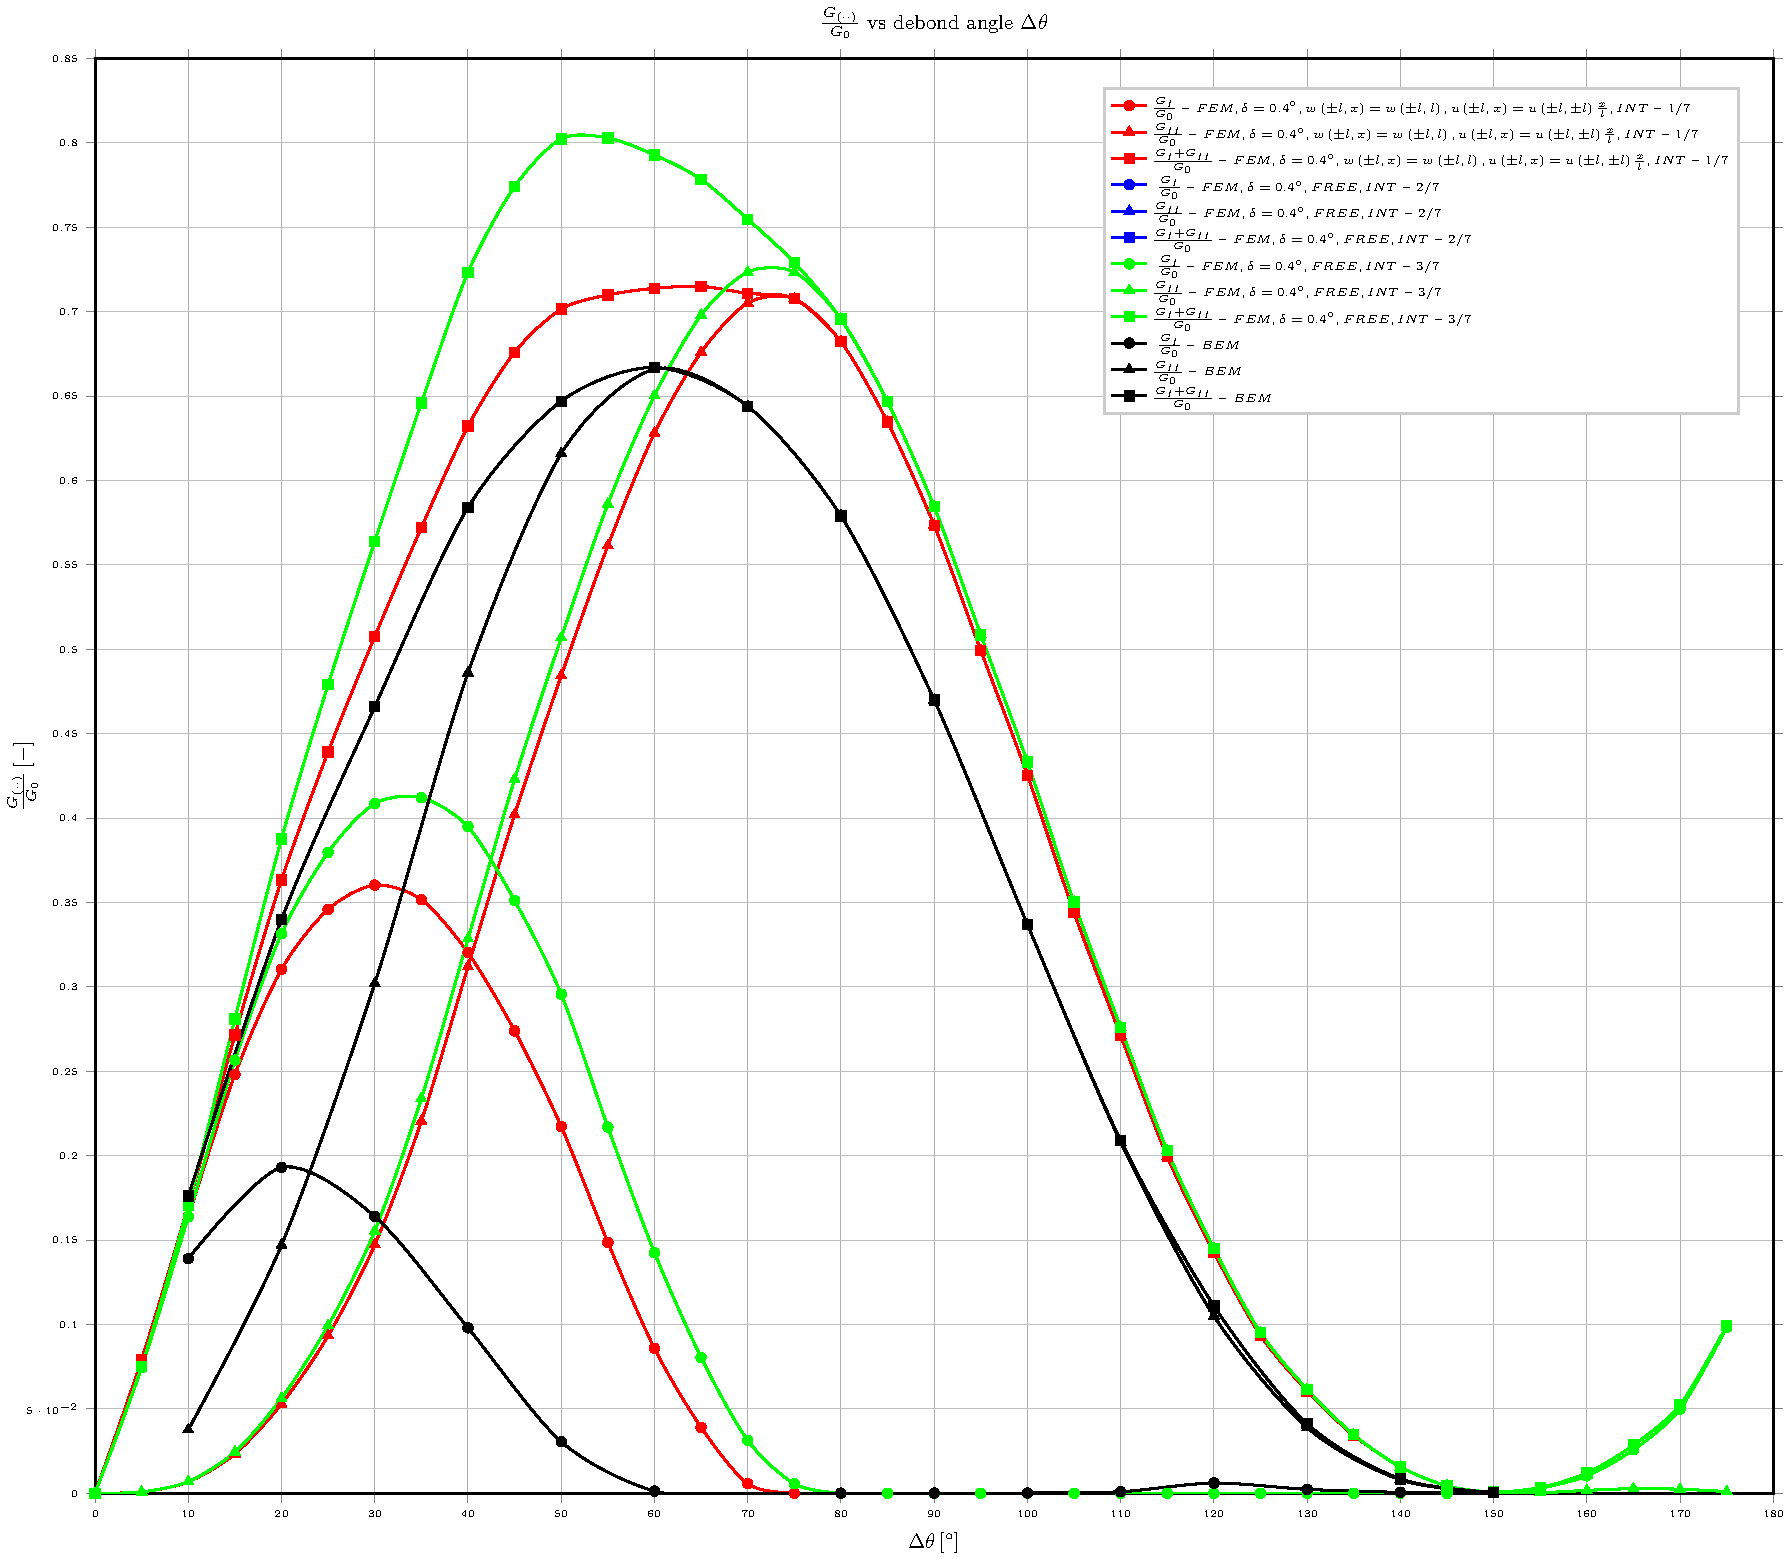
\includegraphics[height=0.7\textheight]{2017-04-29_05-03_AbqRunSummary_GsoverG0_FEM-BEM-comparison.pdf}
  \caption{\scriptsize Formulation de l'interface 2/7 et 3/7.}
  \label{fig:res1}
\end{figure}
\end{frame}

\begin{frame}
\frametitle{R\'esultats}
\vspace{-0.7cm}
\centering
\captionsetup[figure]{font=scriptsize,labelfont=scriptsize}
\begin{figure}[!h]
\centering
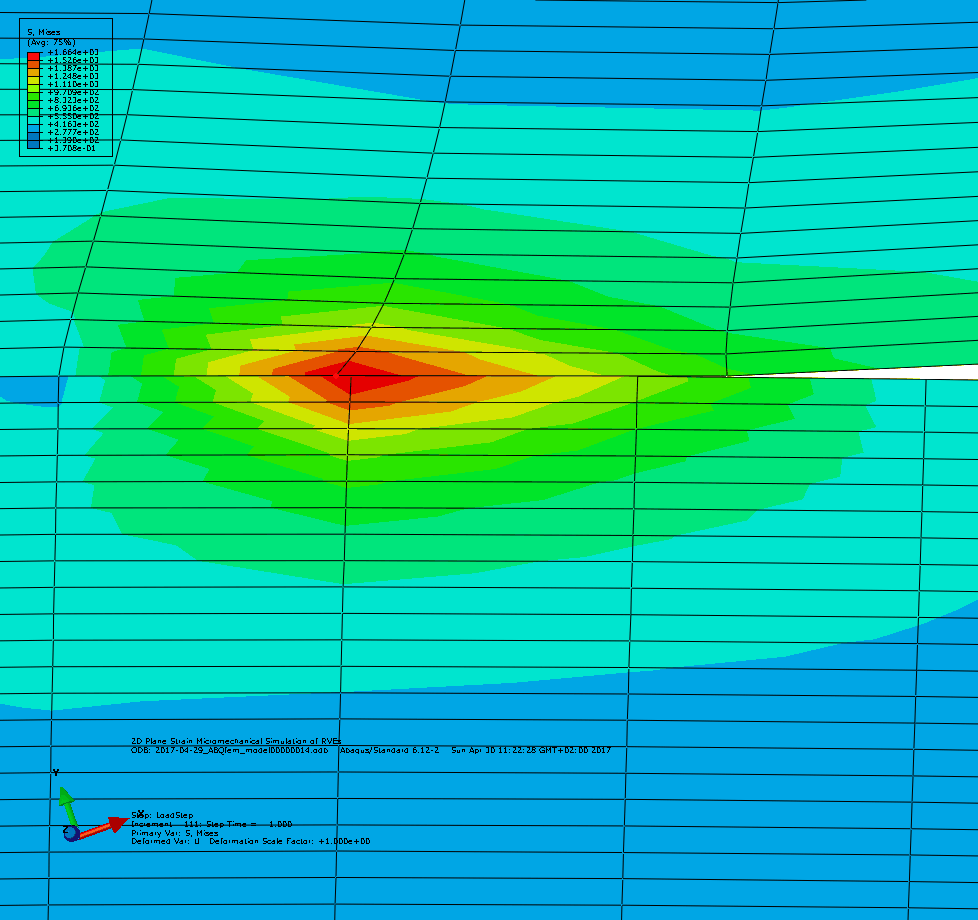
\includegraphics[height=0.7\textheight]{detaille-fissure.png}
  \caption{\scriptsize D\'etail de la fissure pour la formulation 2/7.}
  \label{fig:res1}
\end{figure}
\end{frame}




%\section{Appendices \& References}
%
%\subsection{Appendices}
%
%
%%\end{frame}
%
%\subsection{References}
%
%\begin{frame}[allowframebreaks]
%  \frametitle{References}
%    
%  \begin{thebibliography}{10}
%    
%%  \beamertemplatebookbibitems
%%  % Start with overview books.
%%
%%  \bibitem{Author1990}
%%    A.~Author.
%%    \newblock {\em Handbook of Everything}.
%%    \newblock Some Press, 1990.
% 
%    
%  \beamertemplatearticlebibitems
%  % Followed by interesting articles. Keep the list short. 
%
%\bibitem{DonaldL.Flaggs1982}
%Donald L. Flaggs, Murat H. Kural;
%\newblock {\em Experimental Determination of the In Situ Transverse Lamina Strength in Graphite/Epoxy Laminates.}
%\newblock Journal of Composite Materials, vol. 16, n. 2, 1982.
%
%\bibitem{Parvizi1978}
%Parvizi A., Bailey J.E;
%\newblock {\em On multiple transverse cracking in glass fibre epoxy cross-ply laminates.}
%\newblock Journal of Materials Science, 1978; 13:2131-2136.
%
%\bibitem{herraez2015}
%Miguel Herr\'aez, Diego Mora, Fernando Naya, Claudio S. Lopes, Carlos Gonz\'alez, Javier LLorca;
%\newblock {\em Transverse cracking of cross-ply laminates: A computational micromechanics perspective.}
%\newblock Composites Science and Technology, 2015; 110:196-204.
%
%\bibitem{Canal2012}
%Luis Pablo Canal, Carlos Gonz\'alez, Javier Segurado, Javier LLorca;
%\newblock {\em Intraply fracture of fiber-reinforced composites: Microscopic mechanisms and modeling.}
%\newblock Composites Science and Technology, 2012; 72(11):1223-1232.
%
%\bibitem{StephenW.Tsai2005}
%Stephen W. Tsai;
%\newblock {\em Thin ply composites.}
%\newblock JEC Magazine 18, 2005.
%
%
%\bibitem{ZnedekP.Bazant2002}
%Znedek P. Bazant;
%\newblock {\em Size Effect Theory and its Application to Fracture of Fiber Composites and Sandwich Plates.} 
%\newblock in Continuum Damage Mechanics of Materials and Structures, eds. O. Allix and F. Hild, 2002.
%
%
%\bibitem{RobinAmacherWayneSmithClemensDransfeldJohnBotsis2014}
%Robin Amacher, Wayne Smith, Clemens Dransfeld, John Botsis, Jo\"el Cugnoni;
%\newblock {\em Thin Ply: from Size-Effect Characterization to Real Life Design}
%\newblock CAMX 2014, 2014
%
%\bibitem{RalfCuntze}
%Ralf Cuntze;
%\newblock {\em The  World-Wide-Failure-Exercises -I  and - II for UD-materials.}
%
%
%\bibitem{Pinho}
%Pinho, S. T. and Pimenta, S.;
%\newblock {\em Size Effects on the Strength and Toughness of Fibre-Reinforced Composites.}
%
%\bibitem{PedroP.CamanhoCarlosG.DavilaSilvestreT.PinhoLorenzoIannucci2006}
%Pedro P. Camanho, Carlos G. D\'avila, Silvestre T. Pinho, Lorenzo Iannucci, Paul Robinson;
%\newblock {\em Prediction of in situ strengths and matrix cracking in composites under transverse tension and in-plane shear.}
%\newblock Composites Part A: Applied Science and Manufacturing, vol. 37, n. 2, 2006.
%
%\bibitem{P.P.CamanhoP.Maimi2007}
%P.P. Camanho, P. Maim\'i, C.G. D\'avila;
%\newblock {\em Prediction of size effects in notched laminates using continuum damage mechanics.}
%\newblock Composites Science and Technology, vol. 67, n. 13, 2007.
%
%\bibitem{Nairn1992}
%J. A. Nairn;
%\newblock {\em The Initiation and Growth of Delaminations Induced by Matrix Microcracks in Laminated Composites.}
%\newblock International Journal of Fracture, vol. 57, 1992.
%
%\bibitem{JoelCugnoniRobinAmacher2013}
%Joel Cugnoni , Robin Amacher, John Botsis;
%\newblock {\em Thin ply technology advantages. An overview of the TPT-TECA project.}
%\newblock 2014.
%
%
%  \end{thebibliography}
%\end{frame}

\begin{frame}[plain]
\frametitle{}
\end{frame}

\end{document}

